%!TEX root = ../../Master.tex
\section{Pathfinding Algorithms}

  In \cref{sec:specification} we specified that our solution needs to find the shortest weighted path to the destination.
  To better understanding pathfinding we examined different algorithms. We discovered that some algorithms have a high accuracy but is slow at finding the path, and conversely.
  We have compared some well known path finding algorithms by evaluating their calculation time and route precision.

  In the following we compare 3 frequently used algorithms:
  \begin{itemize}
    \setlength{\itemsep}{1pt}
    \setlength{\parskip}{0pt}
    \setlength{\parsep}{0pt}
    \item \textbf{Dijkstra's Algorithm} Always finds the shortest path but has long calculation time on more complex graphs.
    \item \textbf{Greedy Best-First-Searches} Is a very fast algorithm but does not always find the shortest path.
    \item \textbf{A* Algorithm} Is an extension of Dijkstra's Algorithm but has less calculation time using heuristic values.
\end{itemize}

The A* algorithm was chosen as the algoritm of choice because it always finds the shortest path, and still has a reasonable fast computing time. This algorithm also makes it easier to implement stairs and elevators, because of the heuristic values. In this section we will describe A* and Dijkstra's because A* is an extension of Dijkstra's.


  %Path finding algorithms are used for finding a path between two locations, the source and the destination. By searching its way from the source to the destination, until a path is found. These algorithms also make it possible to calculate the optimal path, i.e. the shortest. \cite{Cormen2009}


  \begin{figure}[ht!]
    \centering
    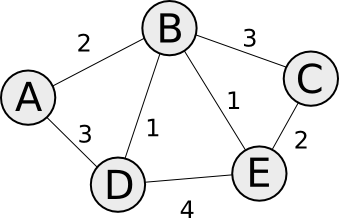
\includegraphics[width=0.5\textwidth]{Graph}
    \caption{Weighted graph}
    \label{fig:graph}
  \end{figure}

  %An important factor of a searching algorithm is correctness and also the time required to calculate the optimized path. The algorithms can be rated by their worst-case time, to ensure a responsive performance.

  \subsection{Dijkstra's Algorithm}


  A commonly used algorithm for finding the shortest path is Dijkstra's algorithm. It loops through steps until all vertices to the target vertex is optimized with the least cost, then points out the shortest path from source vertex, to target vertex. Because of the need of every vertex being evaluated, see \cref{fig:dijkstra}, the complexity of algorithm is proportional to the number of vertices, which means that a lot of computational power is required to calculate the result. \cite{Dijkstr1959}

  \begin{figure}[ht!]
    \centering
    \frame{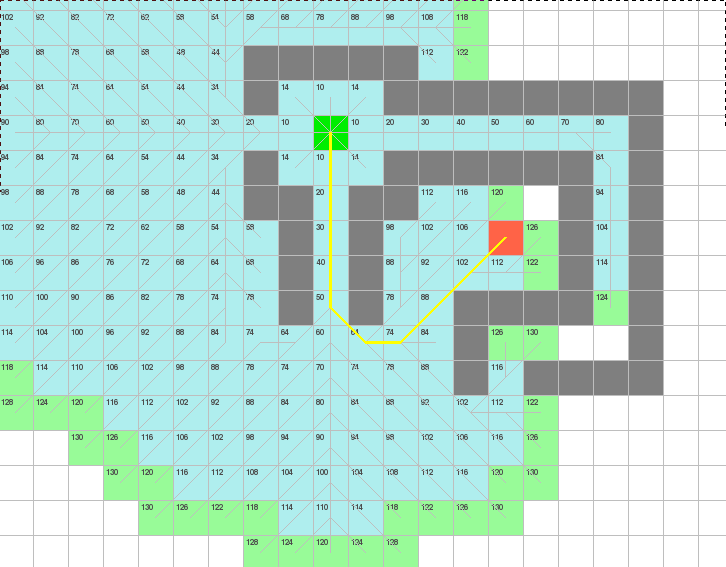
\includegraphics[width=0.5\textwidth]{Dijkstra}}
    \caption{Dijkstra's algorithm in action}
    \label{fig:dijkstra}
  \end{figure}

\begin{algorithm} \label{algo:Dij}
  \caption{Dijkstra's Algorithm}
  \KwResult{Finds the shortest path from start vertex to Vertices}
  \KwData{\\
  graph \tcc*{graph containing vertices}
  source \tcc*{the source vertex to start evaluating from}
  dist \tcc*{list of distances from source}
  visited \tcc*{list of visited vertices}
  previous \tcc*{list of vertices with shortest parent}
  Q \tcc*{A list vertices to be evaluated}
  v \tcc*{evaluating vertex}
  u \tcc*{current vertex}
  }

  \SetKwFunction{Dijkstra}{Dijkstra}
  \SetKwProg{KwFn}{Function}{}{}

  \KwFn{\Dijkstra{graph, source}}{

    \For{\textbf{each} vertex v in graph}{
      dist[$v$] $\gets \infty$\tcc*{Assign distance from source to as infinite}
      visited[$v$] $\gets$ false\tcc*{Boolean to false for not visited}
      previous[$v$] $\gets$ undefined\tcc*{Assign previous all as undefined}
    }

    dist[$source$] $\gets 0$\tcc*{Source dist has distance 0}
    insert $source$ in $Q$\tcc*{Source dist has distance 0}

    \While{Q \textbf{is not} empty}{
      $u \gets$ vertex $v$ in $Q$ with lowest dist[]\tcc*{The new $u$ is the vertex with lowest dist value}
      remove $u$ from $Q$\tcc*{Remove vertex $u$ from $Q$}
      visited[$u$] $\gets$ true\tcc*{Mark the new vertex $u$ as visited}

      \For{\textbf{each} neighbour v of u}{
        $alt \gets$ dist[$u$] + distBetween($v$, $u$)\tcc*{Assign the cost to $v$ from $source$ added the weight between $v$ and $u$}
        \If{alt < dist[v]\tcc*{If $alt$ is lower than the already assign dist value for vertex $v$}}{
          dist[$v$] $\gets alt$\tcc*{Store the shortest distance to vertex $v$ from $source$}
          previous[$v$] $\gets u$\tcc*{Store the short parent $u$ to current vertex $v$}
          \If{!visited[v]}{
            insert $v$ into $Q$\tcc*{Add the unvisited $v$ into the $Q$ to be evaluated}
          }
        }
      }
    }
    return dist\tcc*{Return the distances in dist}
  }
\end{algorithm}

\begin{algorithm} \label{algo:FindPath}
  \caption{Find path to target}
  \KwResult{Finds the shortest path from start vertex to a target vertex}
  \KwData{\\
        stack \tcc*{Empty sequence}
        target \tcc*{Target vertices}
        source \tcc*{Source vertex}
        u \tcc*{evaluating vertices}
        previous \tcc*{A list of parents with lowest cost from source}
   }

  \SetKwFunction{FindPath}{FindPath}
  \SetKwProg{KwFn}{Function}{}{}

  \KwFn{\FindPath{previous, source, target}}{
    $u \gets target$\;
    $stack \gets$ empty sequence\;
    \While{previous[u] \textbf{is not} source}{
      insert $u$ in stack\tcc*{Insert u vertex in the stack}
      $u \gets$ previous[$u$]\tcc*{Traverse from target to source}
    }
    return
  }
\end{algorithm}

  % We consider the problem: find shortest path from source to target.

  % Where $P$ is the source vertex, $Q$ is the target and $R$ is the evaluating vertex.

  % The vertices are subdivided into three sets:

  % \begin{description}
  %   \item[Set $A$]{Optimized vertices (least costly path from $P$ is known)}
  %   \item[Set $B$]{Temporary vertices (evaluated cost of path from $P$ but not part of set $A$)}
  %   \item[Set $C$]{Remaining vertices}
  % \end{description}

  % The edges are subdivided into three other sets:

  % \begin{description}
  %   \item[Set \RN{1}]{Edges used in the set $A$}
  %   \item[Set \RN{2}]{Not part of set I (one and only one edge of this set will lead to each vertex in set $B$)}
  %   \item[Set \RN{3}]{Remaining edges (rejected or not yet considered)}
  % \end{description}

  % At first all vertices is assigned to set $C$ and all edges to set \RN{3}, P is then assigned to set $A$.
  % Then we loop through following steps until $Q$ is part of set $A$. R is the evaluating vertex, and r is the connected edge.

  % \begin{description}
  %   \item[Step 1.]{Consider all the edges r connecting the vertex just assigned to set $A$. If $R$ is part of set $C$ assign to set $B$ and assign edge r to set \RN{2}. If vertex R is part of set $B$, then investigate if the use of edge r is less costly from $P$ to R than the existing edge in set \RN{2}. If less costly assign edge r and reject existing edge in set \RN{2}, otherwise reject r to set \RN{3}.}
  %   \item[Step 2.]{For each vertex in set $B$ where there is only one path in set \RN{1} and set \RN{2}, the vertex with minimum cost from $P$ is assign to set $A$ and with the corresponding edge assign to set \RN{1}.}
  % \end{description}



  % In this example \cref{fig:dijkstra_calc}, the first vertex B is assigned to set $A$, and edge $AB$ is part of set \RN{1}.

  % \begin{figure}[ht!]
  %   \centering
  %   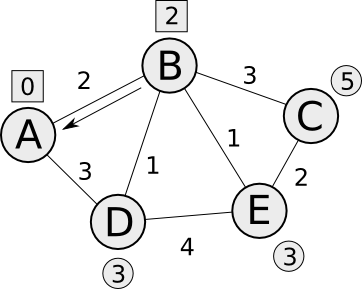
\includegraphics[width=0.5\textwidth]{DijkstraX}
  %   \caption{Dijkstra calculation}
  %   \label{fig:dijkstra_calc}
  % \end{figure}

  \subsection{A* Algorithm}

  If you would combine Dijkstra's algorithm with Best-First-Search algorithm, you would get the A* algorithm which also utilises the principle of a heuristic estimation to determine which vertex to test next. It uses a evaluation function $f(x) = g(x) + h(x)$, where $g(x)$ describes the cost from the start to the vertex being evaluated, and $h(x)$ is a heuristic function that estimates the cost from the evaluating vertex to the target vertex. \cite{Patel2013}

  \begin{itemize}
    \item If $h(x)$ is zero, then only $g$ affects the result and making it work like Dijkstra's algorithm.

    \item If $h(x) < g(x)$, the algorithm will guaranteed find the shortest path from source to target, at a slow running time.

    \item $h(x) = g(x)$, the algorithm will only extract the best path, but this not always possible due to obstacles.

    \item If $h(x) > g(x)$, the algorithm will find a path very fast but not always the optimal, like the Best-First-Search algorithm.
  \end{itemize}

  This means that the heuristic estimation should be reasonable, $h(x)$ should be admissible and not overestimate the distance between the evaluating vertex and the target vertex. But should be just right for the final chosen path to be the optimal path and the for the complexity of the algorithm to be at a minimum. Each step the algorithm evaluates the value of $f(x)$ of each vertex to pick the next vertex with the smallest cost.

  As in the example \cref{astar}, the algorithm expand both paths alternately,x because the $f(x)$ value for each hall shifts as the algorithm progress. 

  \begin{figure}[ht!]
    \centering
    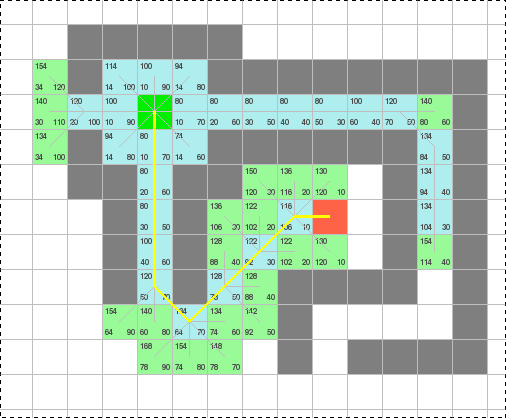
\includegraphics[width=0.5\textwidth]{AstarHlow}
    \caption{A* algorithm with an admissible heuristic value}
    \label{astar}
  \end{figure}

  There are multiple ways to calculate the heuristic value(estimated cost) to the target vertex, but an ideal choice would be the Euclidean \cref{equation:Euclidean} distance, as no path can be shorter than the direct distance between two vertices.
  \begin{equation} \label{equation:Euclidean}
    dist((x, y), (a, b)) = \sqrt{(x - a)^2 + (y - b)^2}
  \end{equation}

  \subsection{Summary of Algorithms}

  Path algorithms searches for a path to target. Some focuses on finding a path fast, others finding the most optimal path. Using the A* algorithm with a heuristic model that is admissible, which underestimates the cost to the target path, assure an optimal path without calculating every vertex. See \cref{tbl:scheme}.
  
  \begin{table}[ht!]
    \centering
  \rowcolors{1}{}{lightgray}
    \begin{tabular}{|r|l|c|}

      \hline
      \textbf{Algorithm} & \textbf{Advantages} & \textbf{Disadvantages} \\
      \hline
      Dijkstra's & Always optimal path & Slow calculation \\
      Best-First-Search & Fast calculation & Not always optimal path \\
      A* & Optimal path if $h(x)<g(x)$, Fast calculation & Not always optimal path \\
      \hline
    \end{tabular}
    \caption{Table of advantages/disadvantages of different algorithms}
    \label{tbl:scheme}
  \end{table}